\documentclass{beamer}
\usetheme{metropolis}           % Use metropolis theme
\definecolor{goethe_blau}{HTML}{00618F} % define goethe color
\setbeamercolor{frametitle}{bg=goethe_blau}
\setbeamercolor{alerted text}{fg=goethe_blau} % use goethe color


%\usepackage[
%    backend=biber,
%    style=apa,
%  ]{biblatex}
%\addbibresource{presentation/bibliography.bib}

\titlegraphic{
\includegraphics[width=2.5cm]{presentation/images/GoetheLogo.png}}

%\logo{{
\includegraphics[width=2cm]{presentation/images/GoetheLogo.png}}\hspace*{1cm}}

\usepackage{caption}

\title{Assembly of long, error-prone reads using repeat graphs}
\date{July 5, 2021}
\author{Mikhail Kolmogorov, Jeffrey Yuan, Yu Lin and Pavel A. Pevzner}
\institute{Presented by: Johannes Hausmann, Luis Kress}


\begin{document}
  \maketitle
  
  %\section{First Section}
  
  \begin{frame}{Background}
    \begin{itemize}[<+- | alert@+>]
      \item Assembly: reconstruct target sequence from the reads

      \item Different assemblers, different graph structures

      \item Repeats $\rightarrow$ assembly fragmentation
      \begin{figure}
        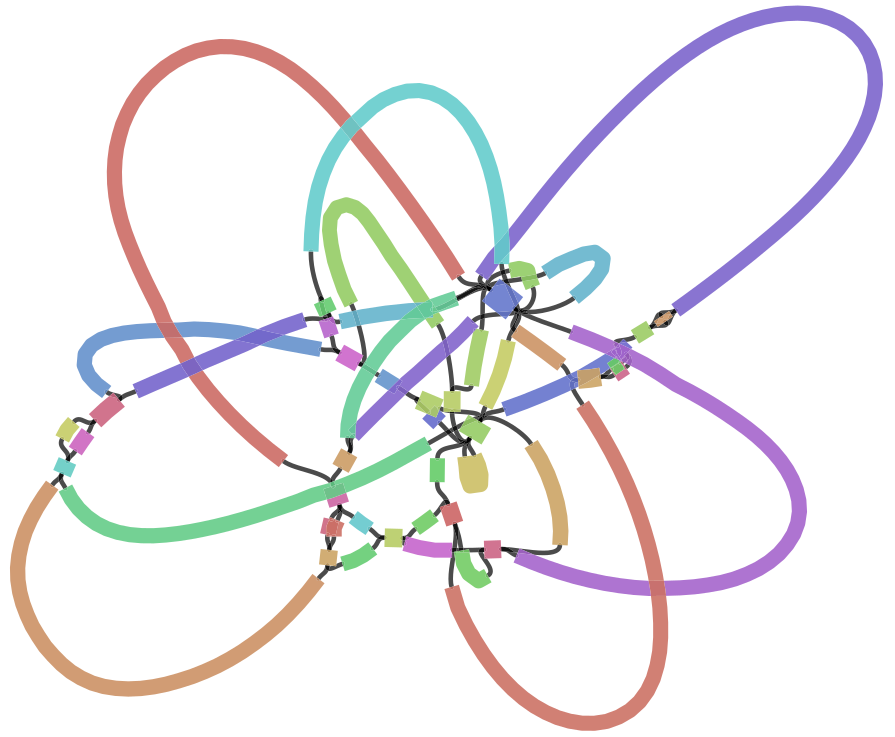
\includegraphics[width=3cm]{presentation/images/tangled.png}
        \caption*{Tangled assembly graph of \textit{E.coli} \cite{kolmogorov_assembly_2019}}
        \label{fig:tangled}
      \end{figure}

      \item Small differences between repeat copies $\rightarrow$ hard to
      resolve with error-prone reads

    \end{itemize}
  \end{frame}

  
  %\begin{frame}{Aim}
  %  \begin{itemize}[<+- | alert@+>]
  %    \item correct resolvation of repetetive regions
  %    \item assemble the long error-prone reads correctly
  %    \item create contiguous assembly
  %  \end{itemize}
  %\end{frame}

  %\section{Second Section}

  \begin{frame}{Disjointigs}
    \begin{itemize}[<+- | alert@+>]
      \item Most assemblers spend much time on correct contig assembly

      \item Flye uses a different approach \cite{kolmogorov_assembly_2019}:
      
      \begin{itemize}[<+- | alert@+>]
        \item we don't care about the correct contig assembly \only<4>{(at least at the initial stage)}
        \begin{figure}
          %\captionsetup{labelformat=empty}
          
\includegraphics[width=2.5cm]{presentation/images/orly-owl.jpg}
          %\caption{Orly}
          \label{fig:orly}
        \end{figure}
        
      %  \item correct assembly graph 
      \end{itemize}

      \item Generate arbitary paths from overlapping reads $\rightarrow$ Disjointigs
    \end{itemize}
  \end{frame}

  \begin{frame}{Repeat Graph Creation}
    \begin{figure}
      %\captionsetup{labelformat=empty}
      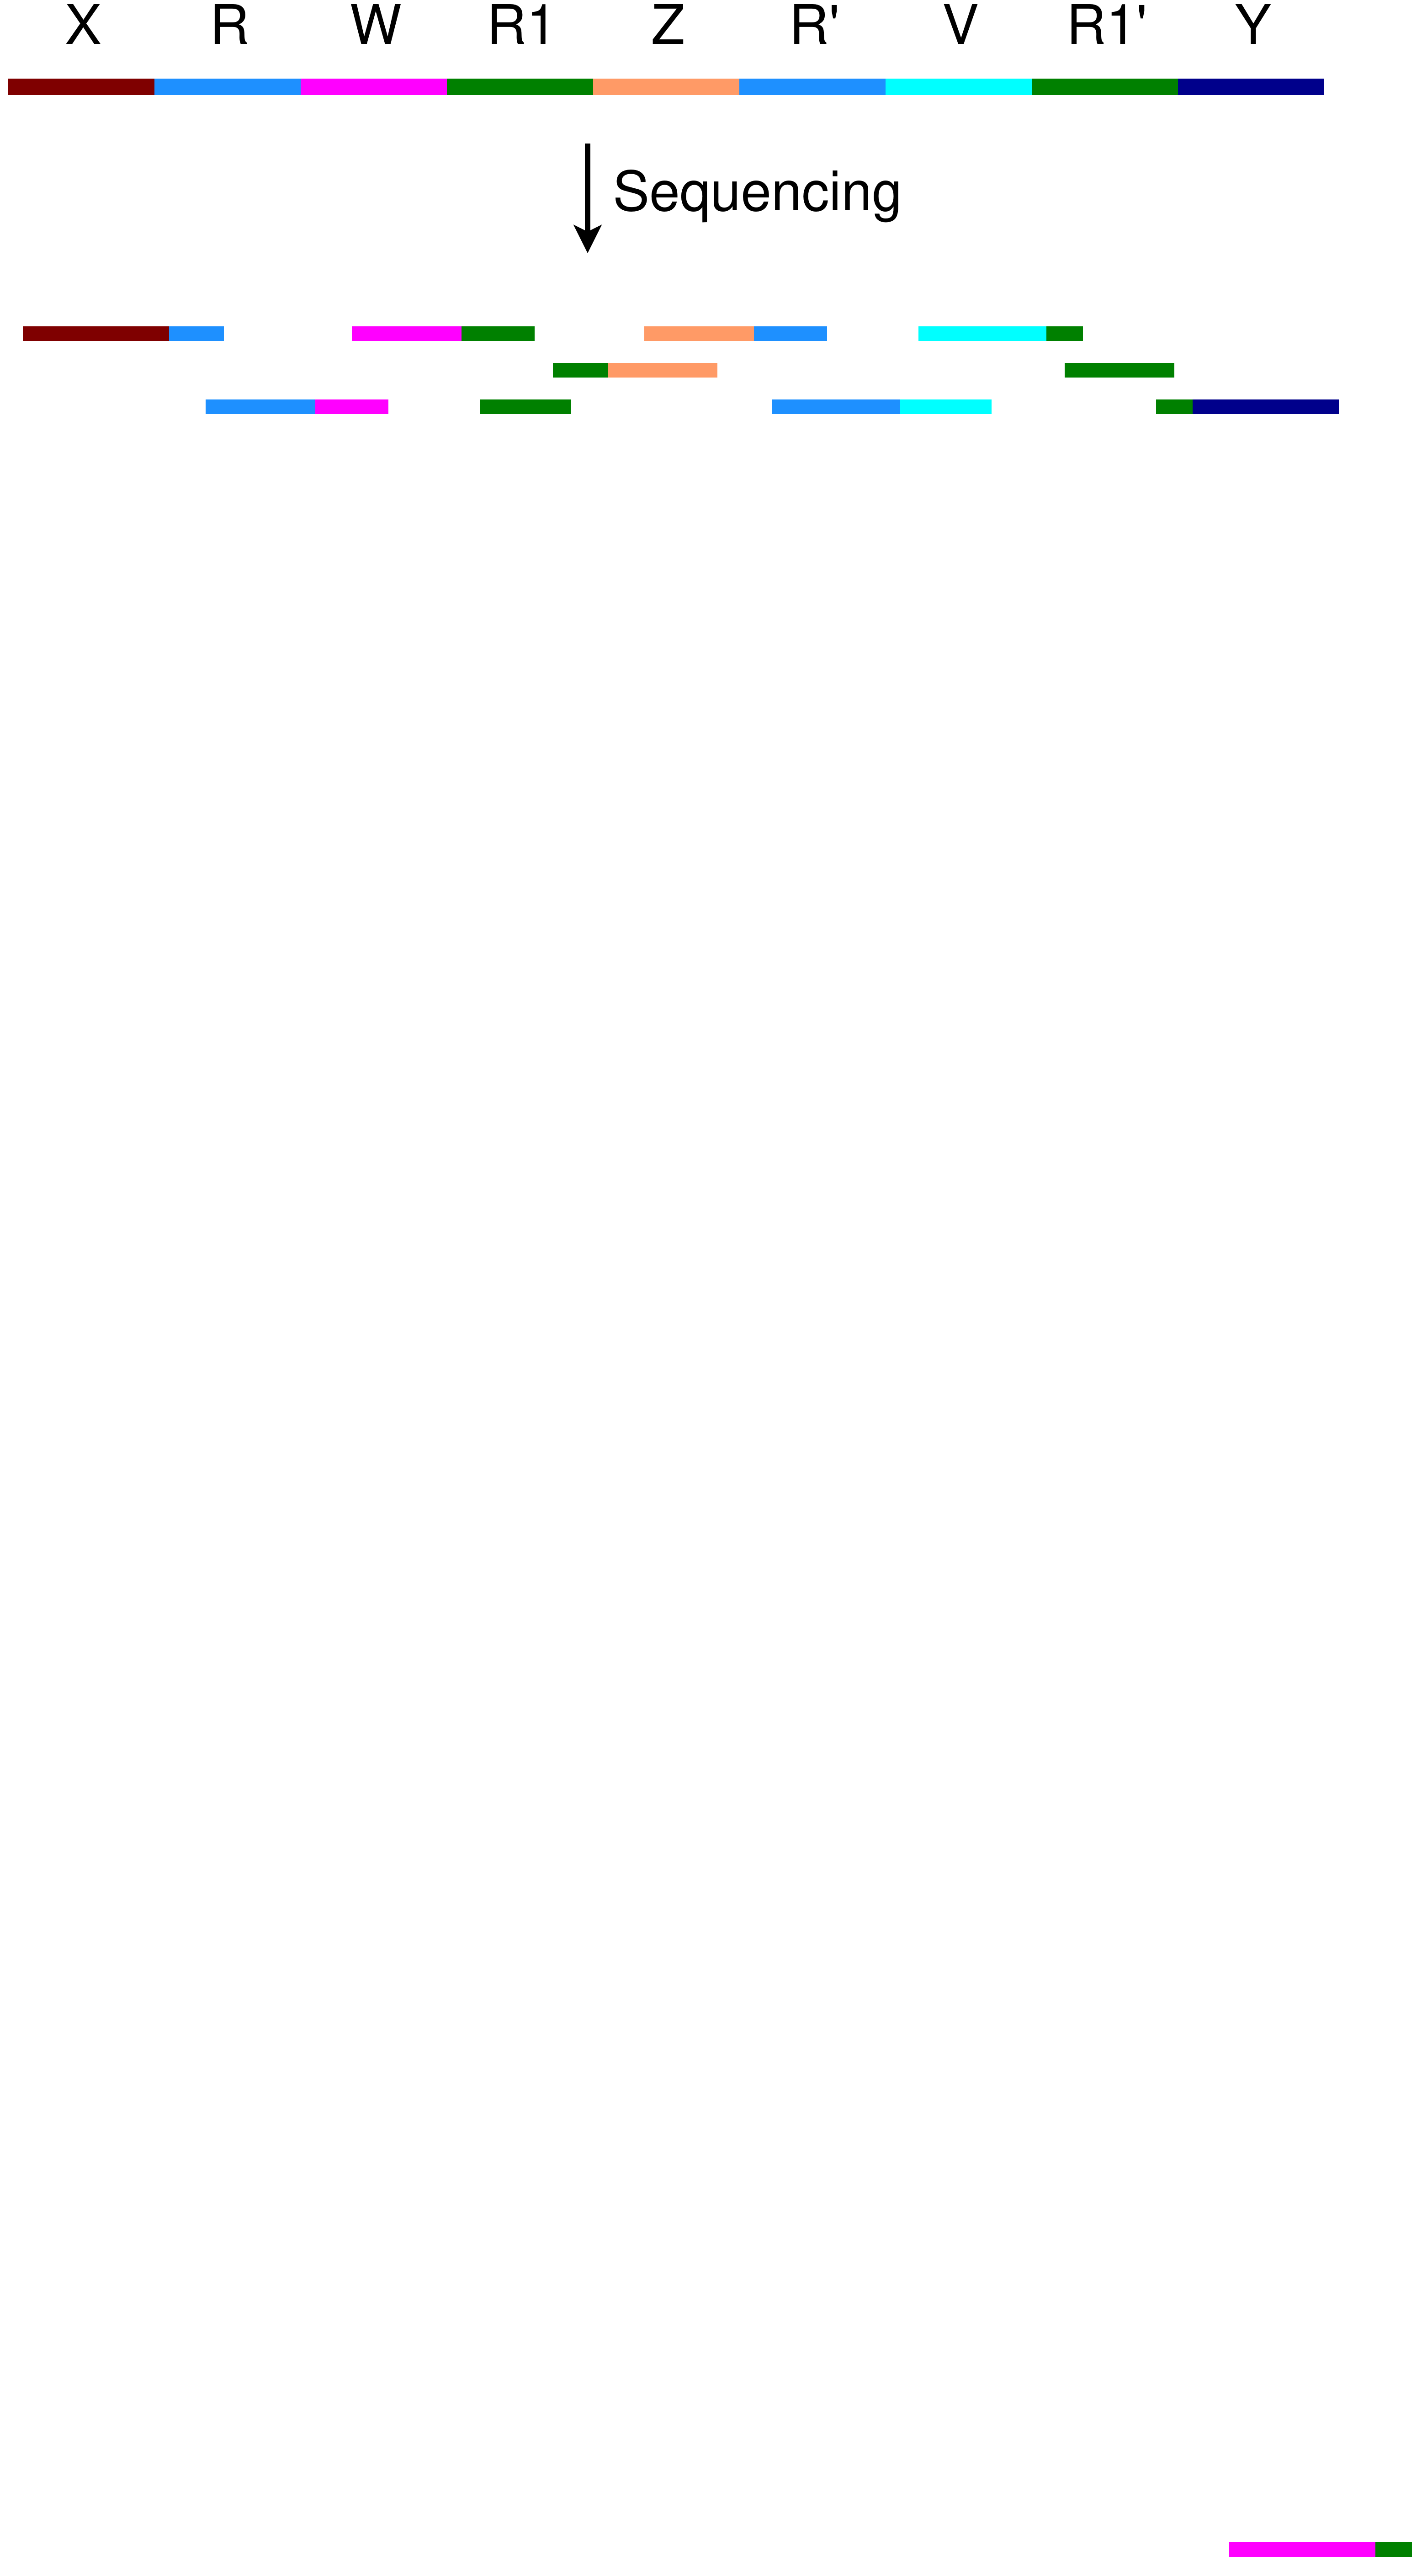
\includegraphics[width=11cm]{presentation/images/genome.png}
      %\caption{Example Genome and Reads}
      \label{fig:genome_and_reads}
    \end{figure}
  \end{frame}

  \begin{frame}{Repeat Graph Creation}
    \begin{figure}
      %\captionsetup{labelformat=empty}
      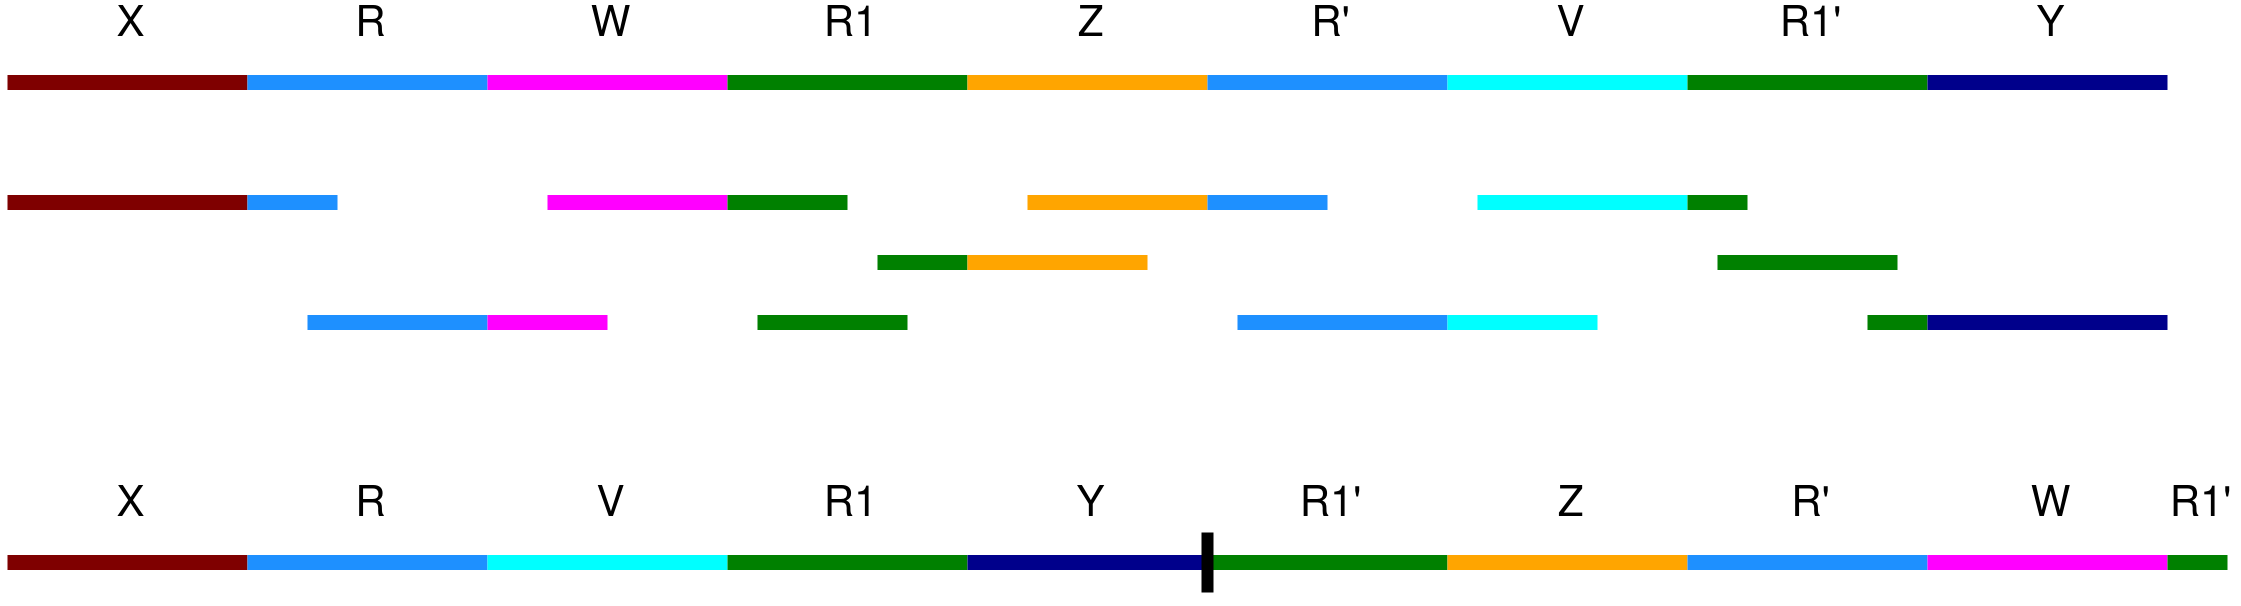
\includegraphics[width=11cm]{presentation/images/disjointigs.png}
      %\caption{Example Genome, Reads and Disjointigs}
      \label{fig:disjointigs}
    \end{figure}
  \end{frame}

  \begin{frame}{Repeat Graph Creation}
    \begin{figure}
      %\captionsetup{labelformat=empty}
      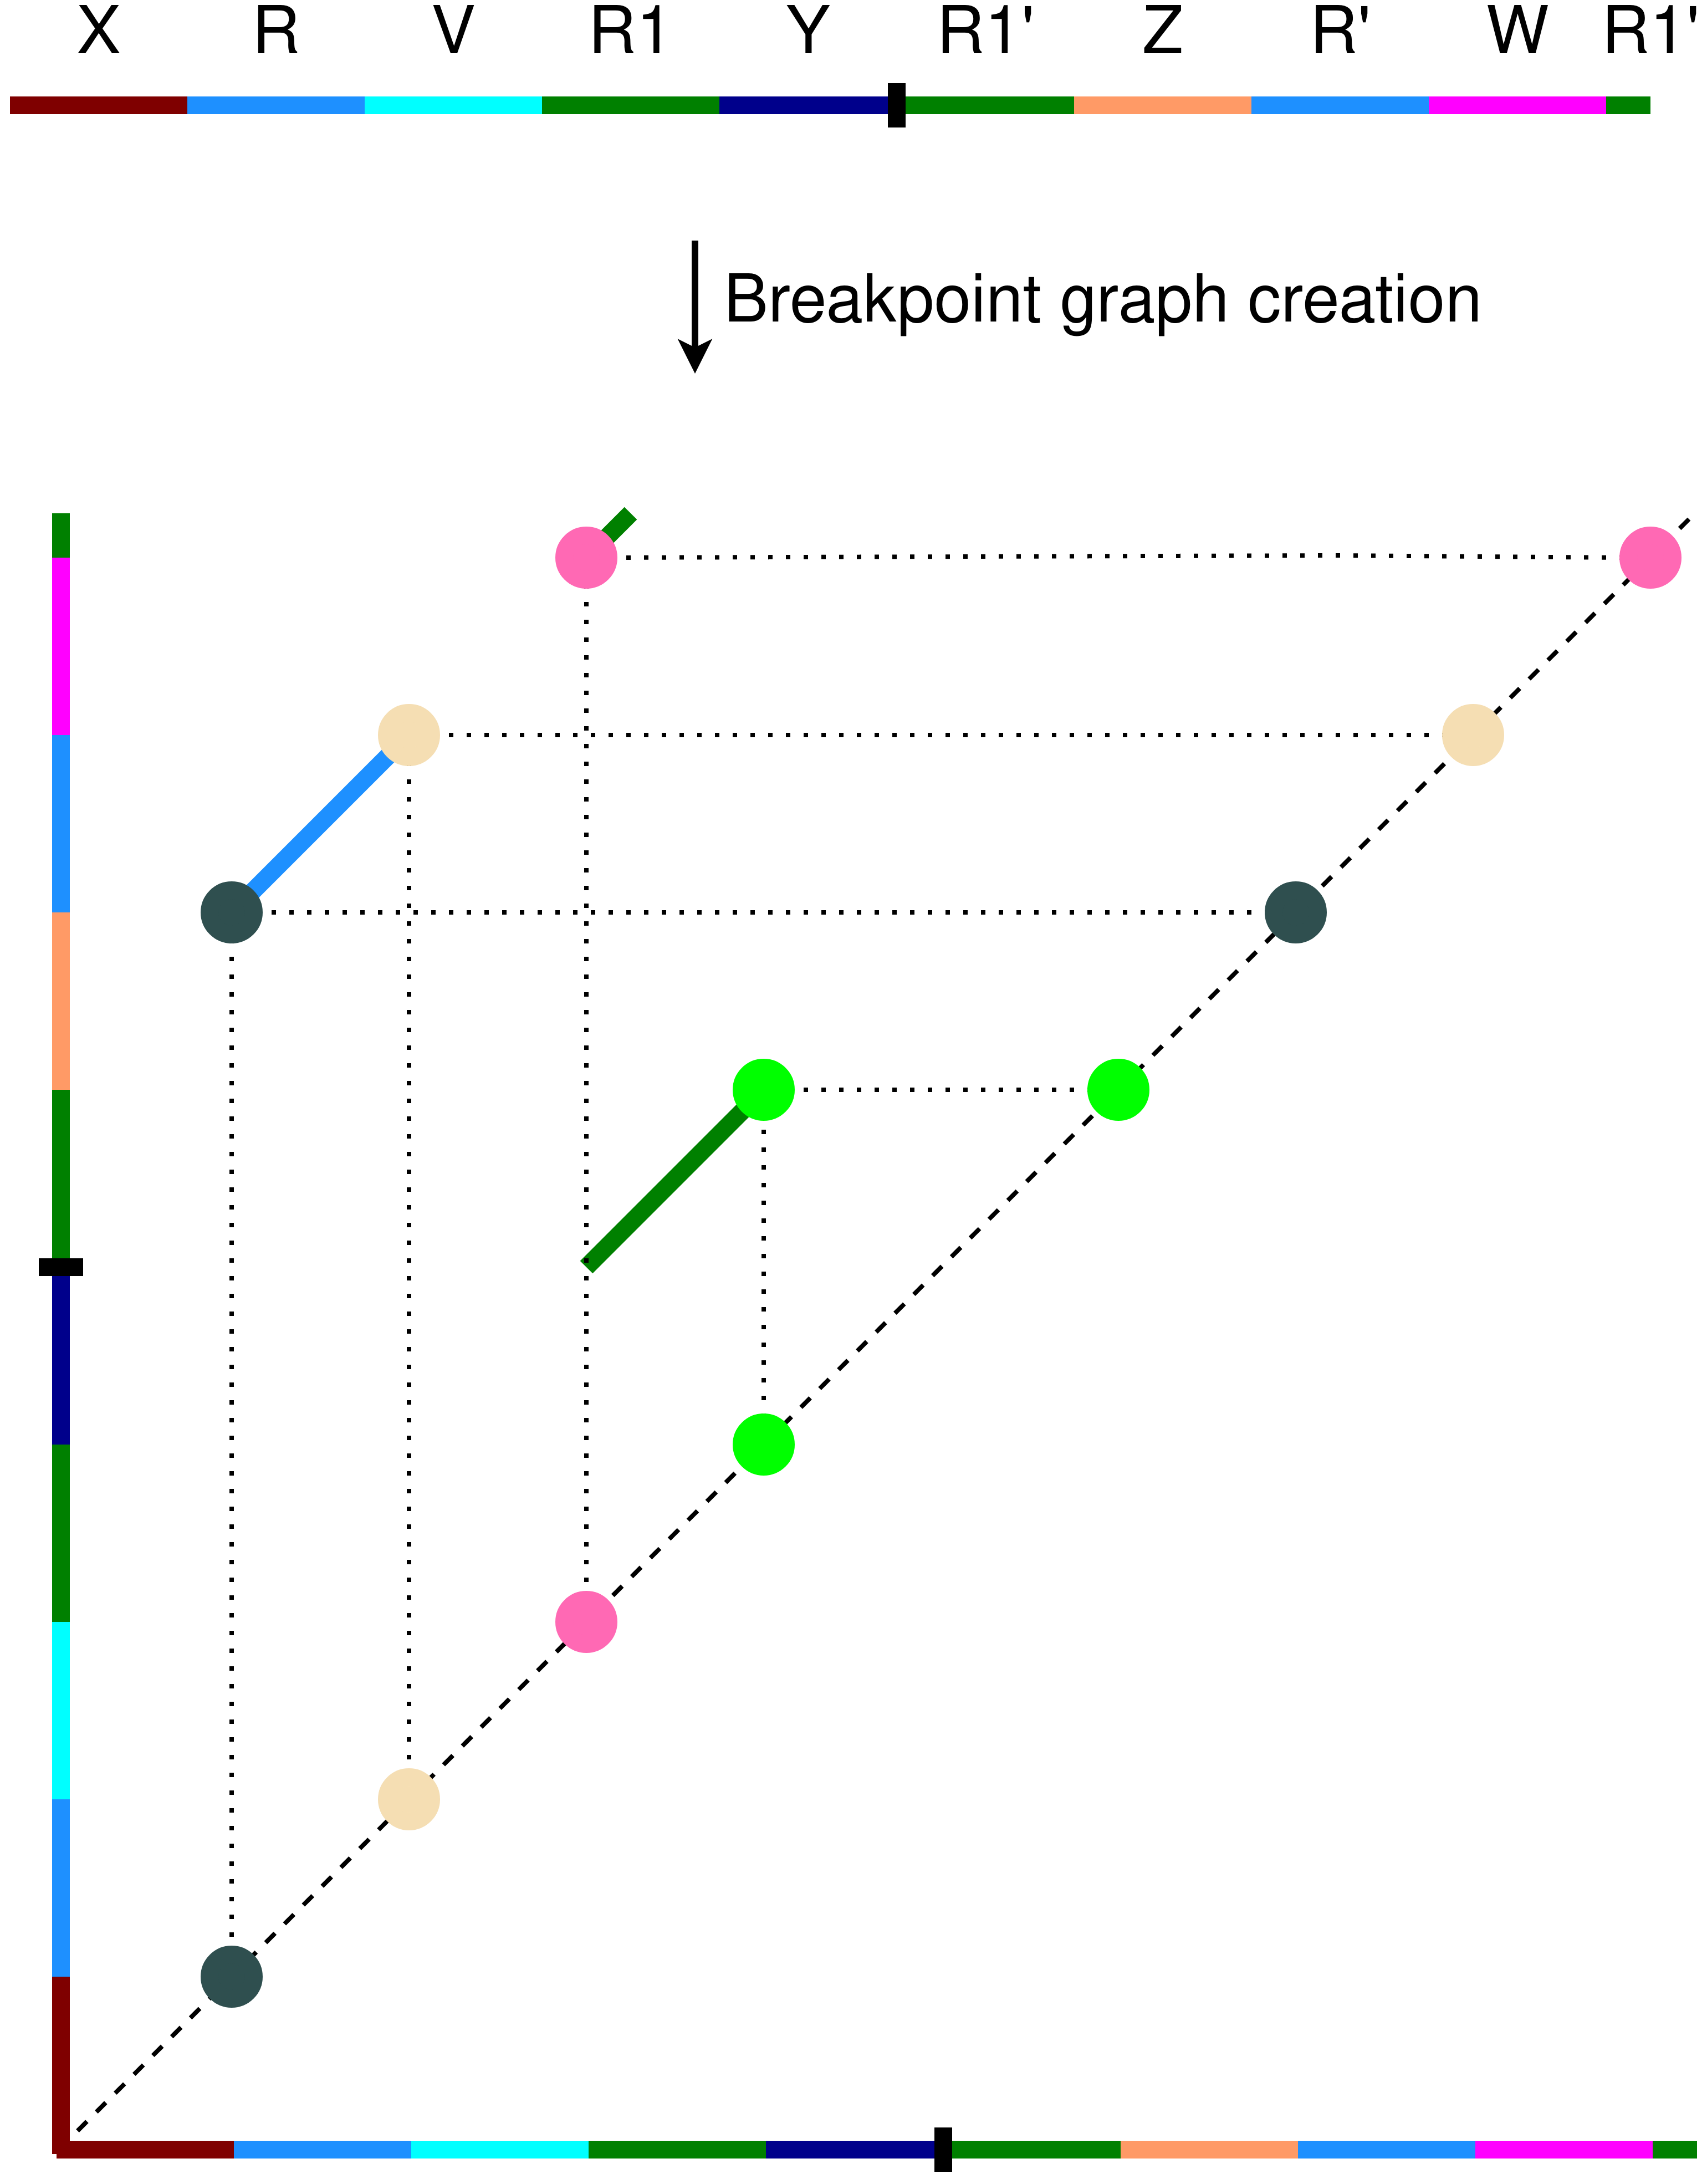
\includegraphics[width=6cm]{presentation/images/breakpoint_graph.png}
      %\caption{Breakpoint Graph}
      \label{fig:bp_graph}
    \end{figure}
  \end{frame}

  \begin{frame}{Repeat Graph Creation}
    \begin{figure}
      %\captionsetup{labelformat=empty}
      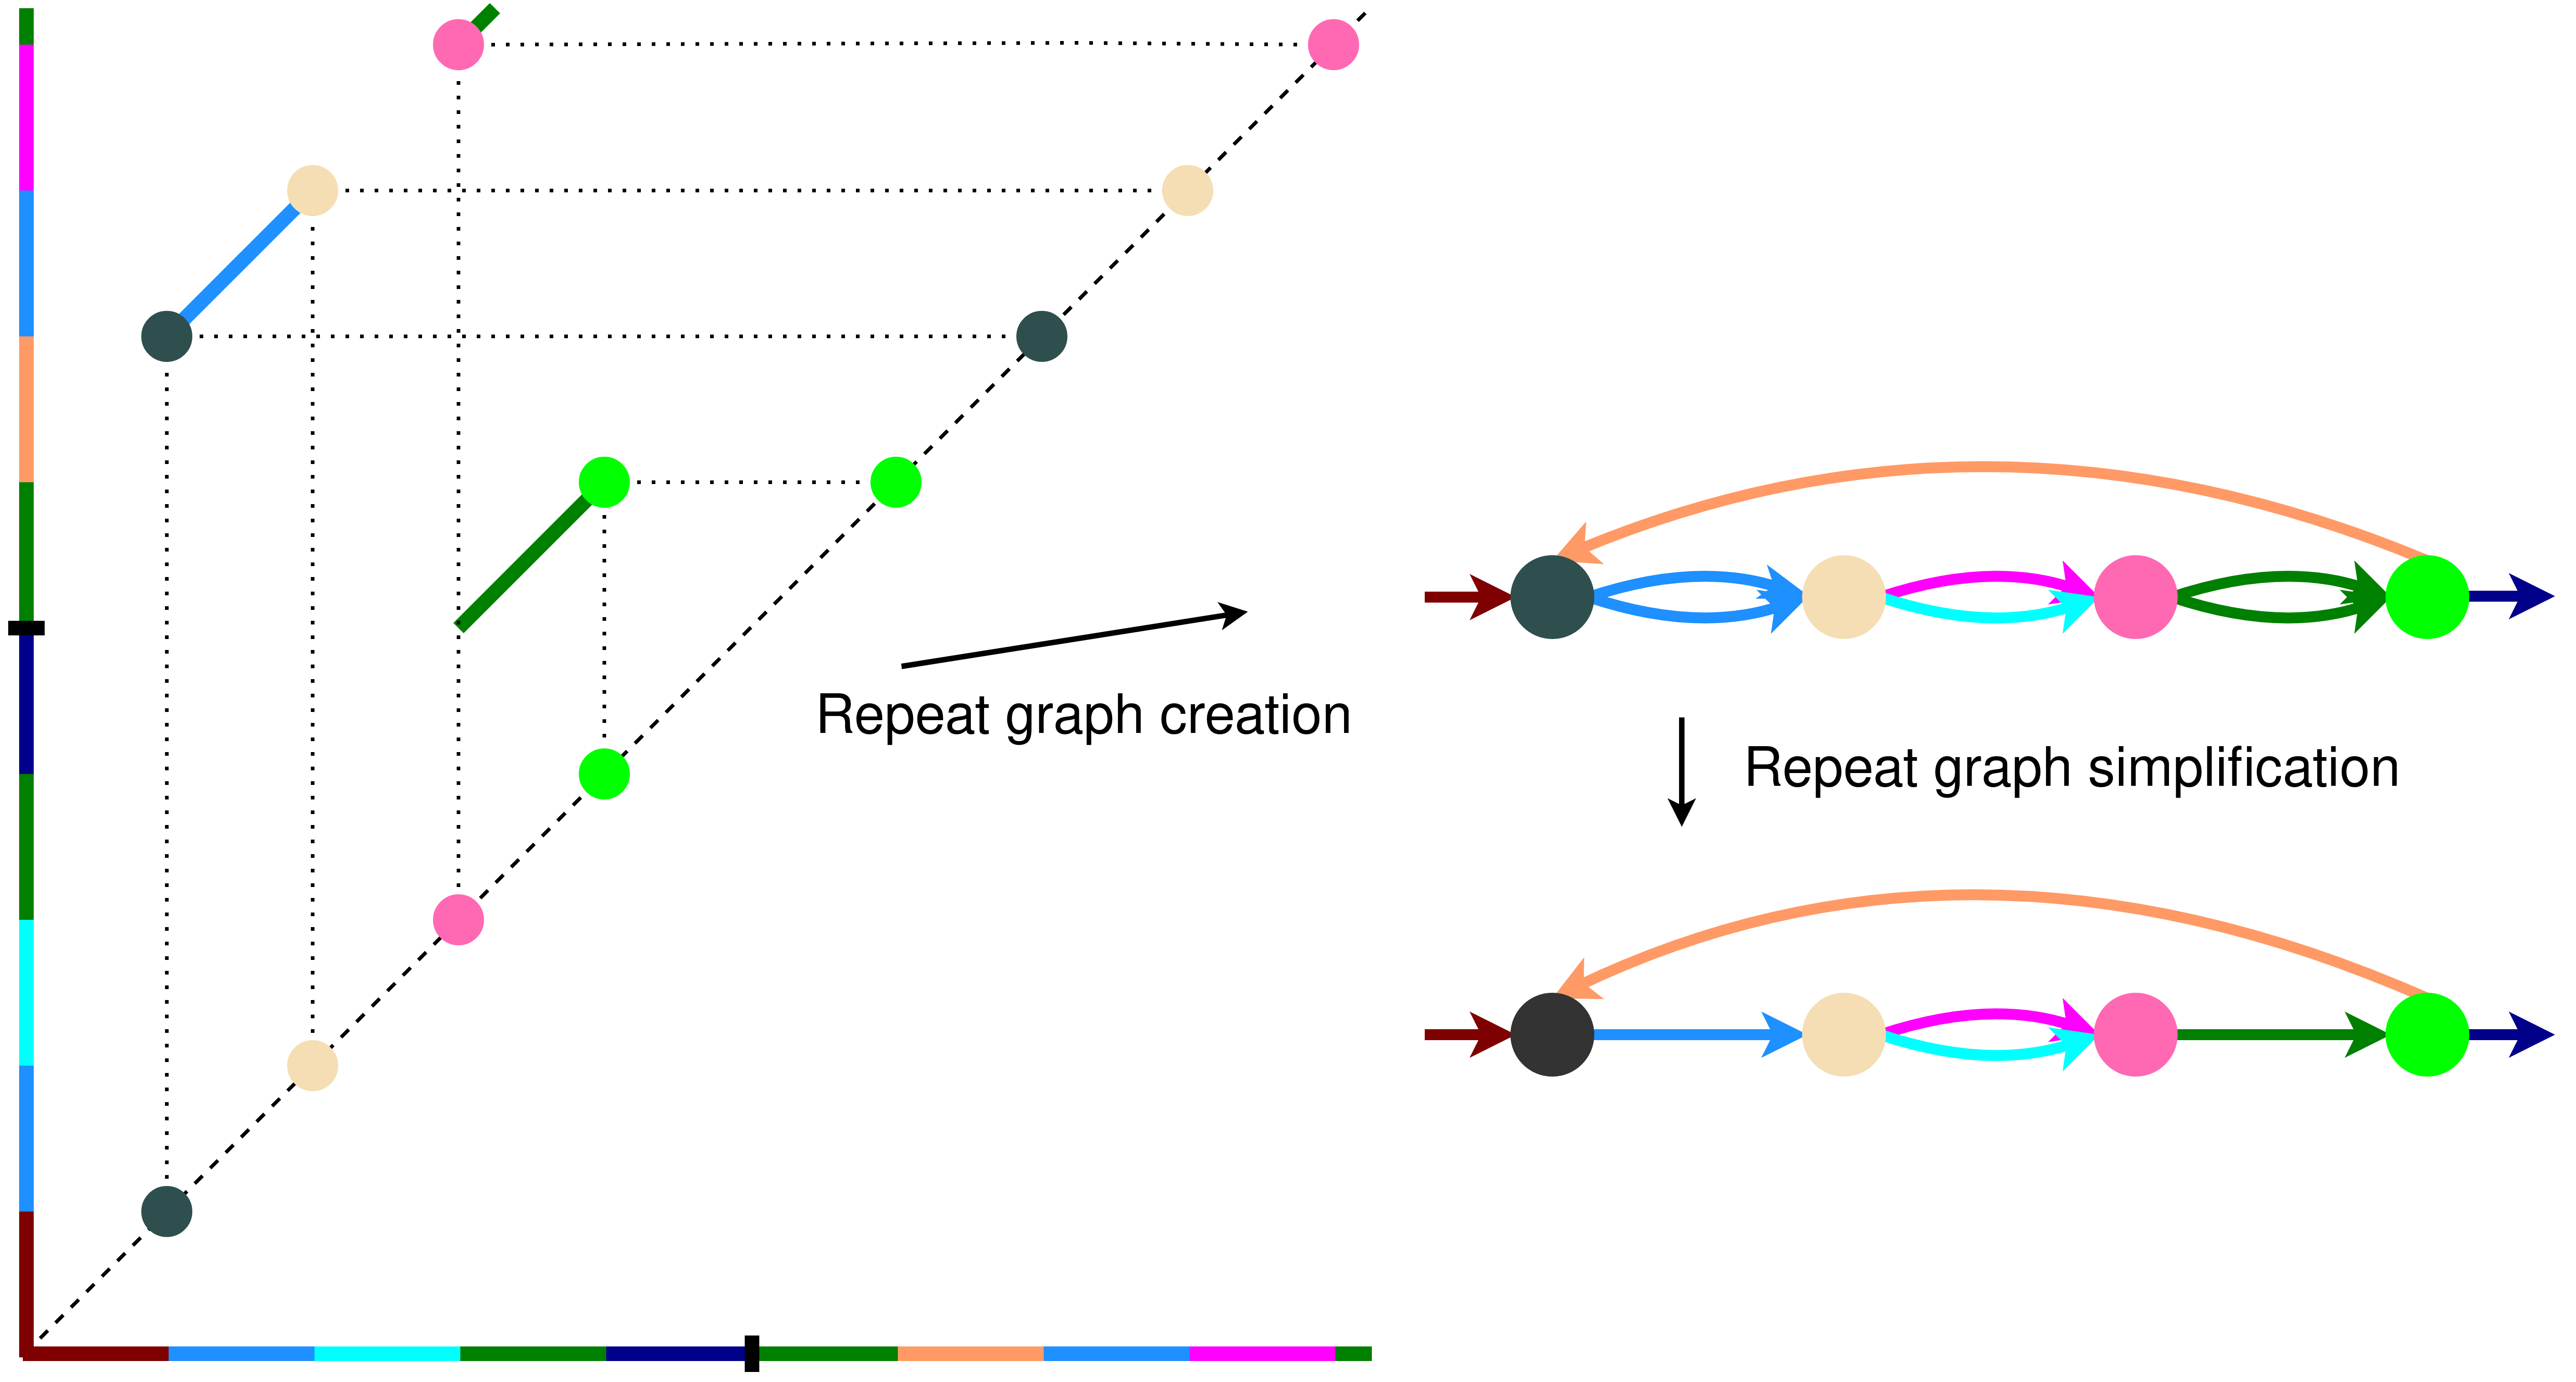
\includegraphics[width=11cm]{presentation/images/repeat_graph.png}
      %\caption{Repeat Graph}
      \label{fig:repeat_graph}
    \end{figure}
  \end{frame}

  \begin{frame}{Results}
    \begin{figure}
      \includegraphics[width=11cm]{presentation/images/results_HUMAN.png}
      \caption{Results for HUMAN testset}
      \label{fig:results}
    \end{figure}
  \end{frame}

  \begin{frame}{Git (presentation and poster)}
    \begin{figure}
      %\captionsetup{labelformat=empty}
      
\includegraphics[width=6cm]{presentation/images/qr-code.png}
      \caption*{https://github.com/LKress/ASA}
      \label{fig:qr}
    \end{figure}
  \end{frame}

  \appendix


  \begin{frame}[allowframebreaks]{References}
    %\begin{small} 
    %  dir: \thepwd
    %\end{small}}
    %{\small dir: \thepwd \par}
    \nocite{walker_pilon_2014}
    %\printbibliography
    \bibliography{literature/bibliography.bib}
    \bibliographystyle{abbrv}
  
  \end{frame}

  \maketitle

  \begin{frame}[standout]
    Appendix
  \end{frame}

  \begin{frame}{Dot plot creation}
    \begin{figure}
      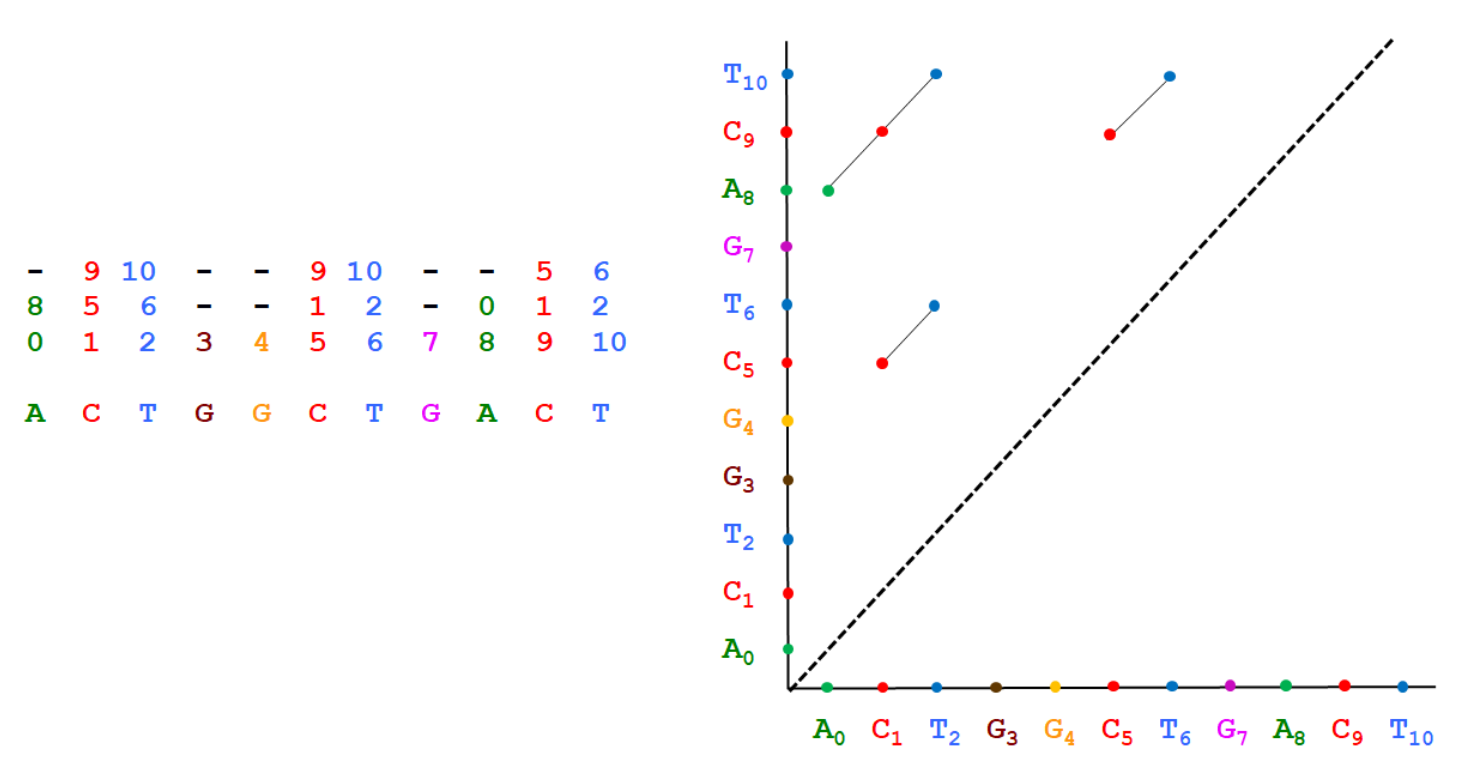
\includegraphics[width=11cm]{presentation/images/dot_plot_creation.png}
      \caption*{Dot plot creation \cite{kolmogorov_assembly_2019}}
      \label{fig:dotp_creation}
    \end{figure}
  \end{frame}

  \begin{frame}{Repeat graphs}
    \begin{itemize}
      \item generalization of de Bruijn graphs

      \item structure

      \item creation
      
      \begin{itemize}

        \item from disjointigs = random walk of reads on the repeat graph 
      
        \item means the repeat graph hasn't to be known
        \item set of disjointigs of a genome is complete if each k+1-mer from the genome is present in a disjointig from this set $\rightarrow$ repeat graph conctruction of complete set of disjointigs same result as repeat graph construction of the genome
      \end{itemize}
    \end{itemize}
  \end{frame}

  \begin{frame}{Difference repeat graph de Bruijn graph}
    \begin{itemize}
      \item A-Bruijn graph (alignments) generalizes the de Bruijn graph

      \item "We thus argue that the time has come to explain that the breakpoint graphs and the de Bruijn graphs are two identical data structures (if one ignores a cosmetic difference between them) as they both represent specific instances of a general notion of the A-Bruijn graph introduced in \cite{lin_what_2014}. The A-Bruijn graphs are based on representing genomes as sets of labeled paths and further gluing identically labeled edges (breakpoint graphs) or vertices (de Bruijn graphs) in the resulting paths." \cite{pevzner_novo_2004}

      \item de Bruijn graphs need correct bases
      
      \item otherwise tangled graph
    \end{itemize}
  \end{frame}

  \begin{frame}{Segmental duplications}
    \begin{figure}
      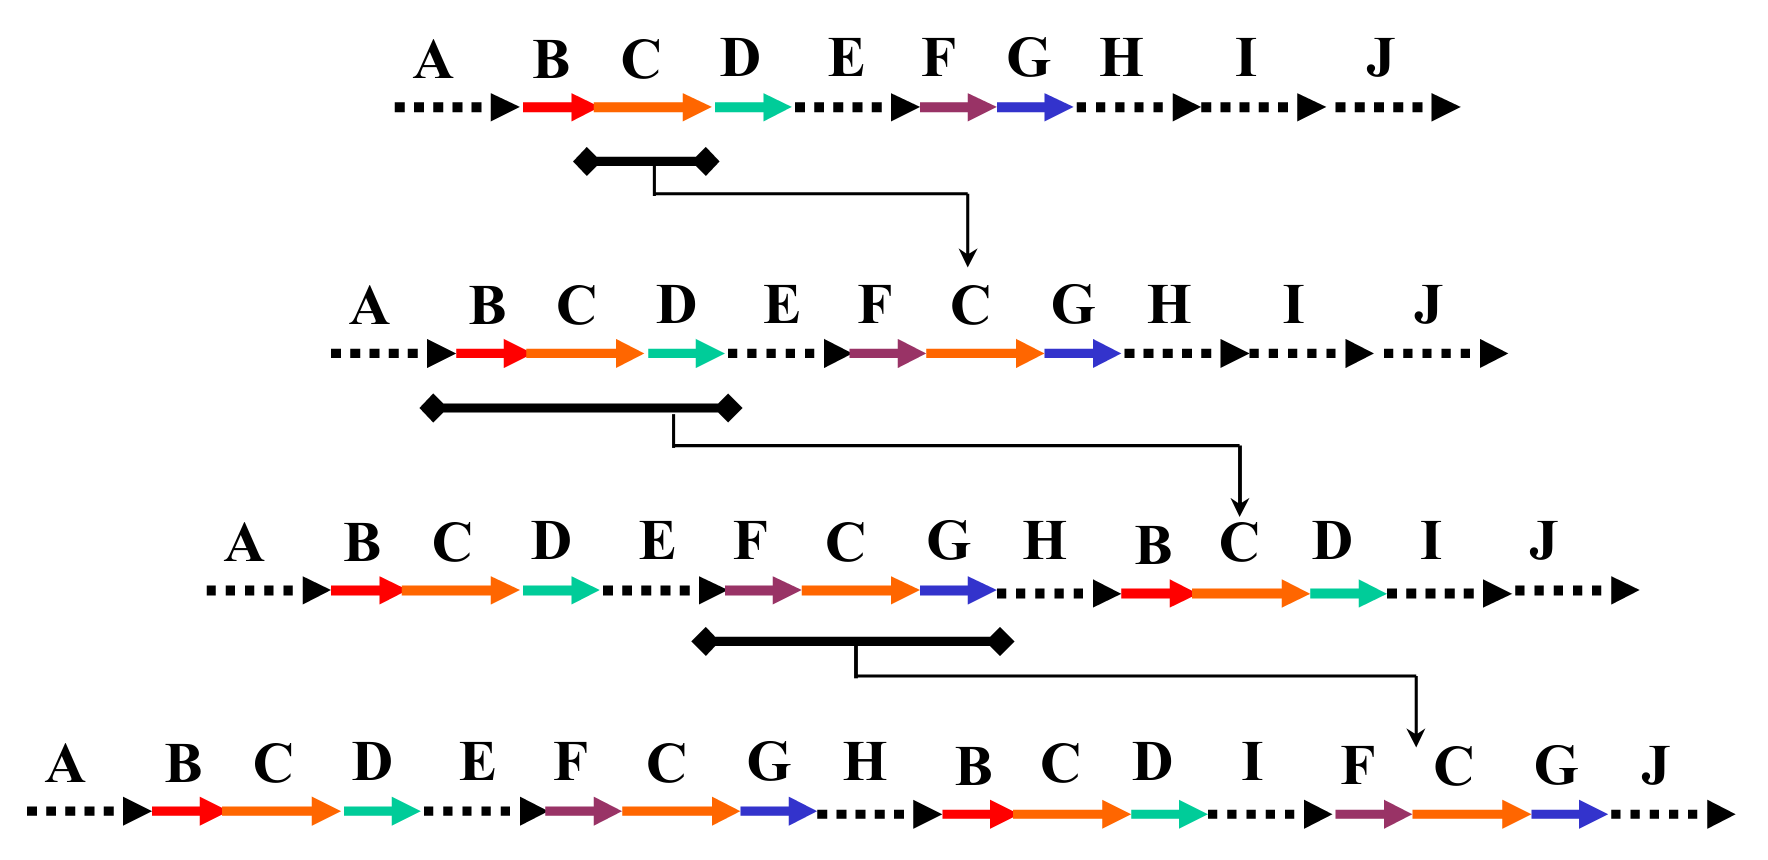
\includegraphics[width=6cm]{presentation/images/SDs.png}
      \caption*{Segmental Duplications \cite{pevzner_novo_2004}}
      \label{fig:SD}
    \end{figure}
    \begin{itemize}
      \item Segmental duplications are duplicated blocks of genomic DNA typically ranging in size from 1-200 kb (IHGSC 2001)

      \item They often contain sequence features such as high-copy repeats and gene sequences with intron-exon structure. 
    \end{itemize}
  \end{frame}

  \begin{frame}{Disjointig creation}
    \begin{figure}
      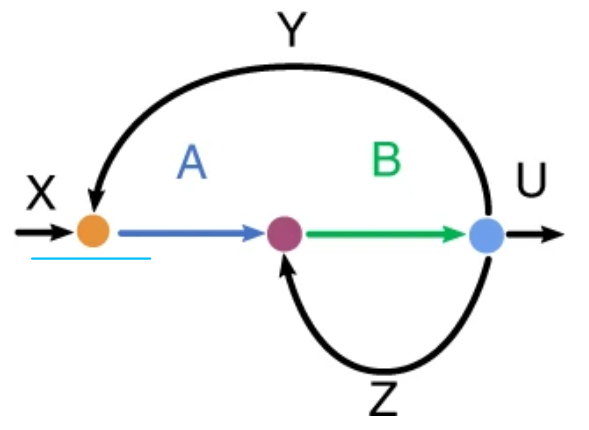
\includegraphics[width=7cm]{presentation/images/repeat_graph_dot1.png}
      %\caption*{}
      \label{fig:repgraph1}
    \end{figure}
    %From: 
    %https://www.youtube.com/watch?v=z6elrX-ZzW8&t=636s
    %(Youtube nanopore talk)
  \end{frame}

  \begin{frame}{Disjointig creation}
    \begin{figure}
      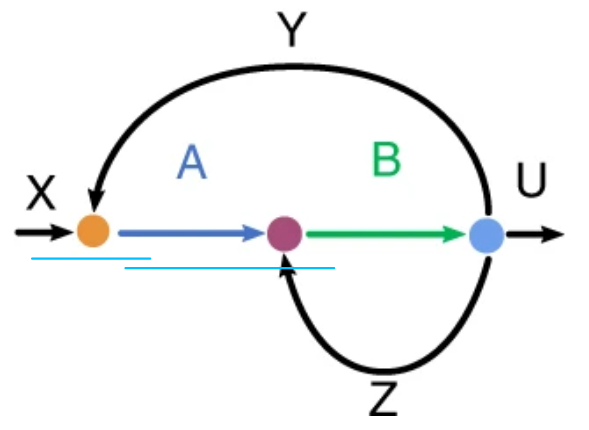
\includegraphics[width=7cm]{presentation/images/repeat_graph_dot2.png}
      %\caption*{}
      \label{fig:repgraph2}
    \end{figure}
    %From: 
    %https://www.youtube.com/watch?v=z6elrX-ZzW8&t=636s
    %(Youtube nanopore talk)
  \end{frame}

  \begin{frame}{Disjointig creation}
    \begin{figure}
      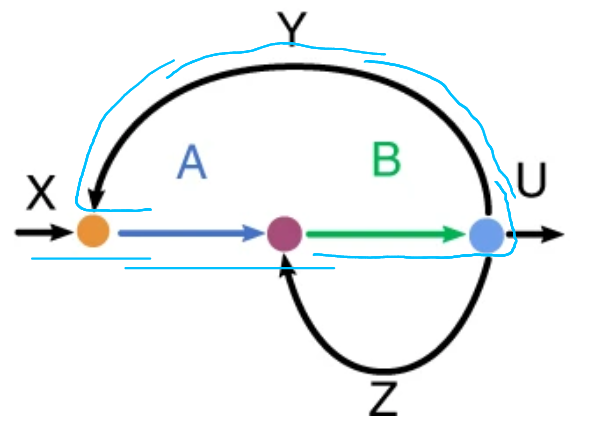
\includegraphics[width=7cm]{presentation/images/repeat_graph_dot3.png}
      %\caption*{}
      \label{fig:repgraph3}
    \end{figure}
    %From: 
    %https://www.youtube.com/watch?v=z6elrX-ZzW8&t=636s
    %(Youtube nanopore talk)
  \end{frame}

  \begin{frame}{Repeat resolution}
    \begin{figure}
      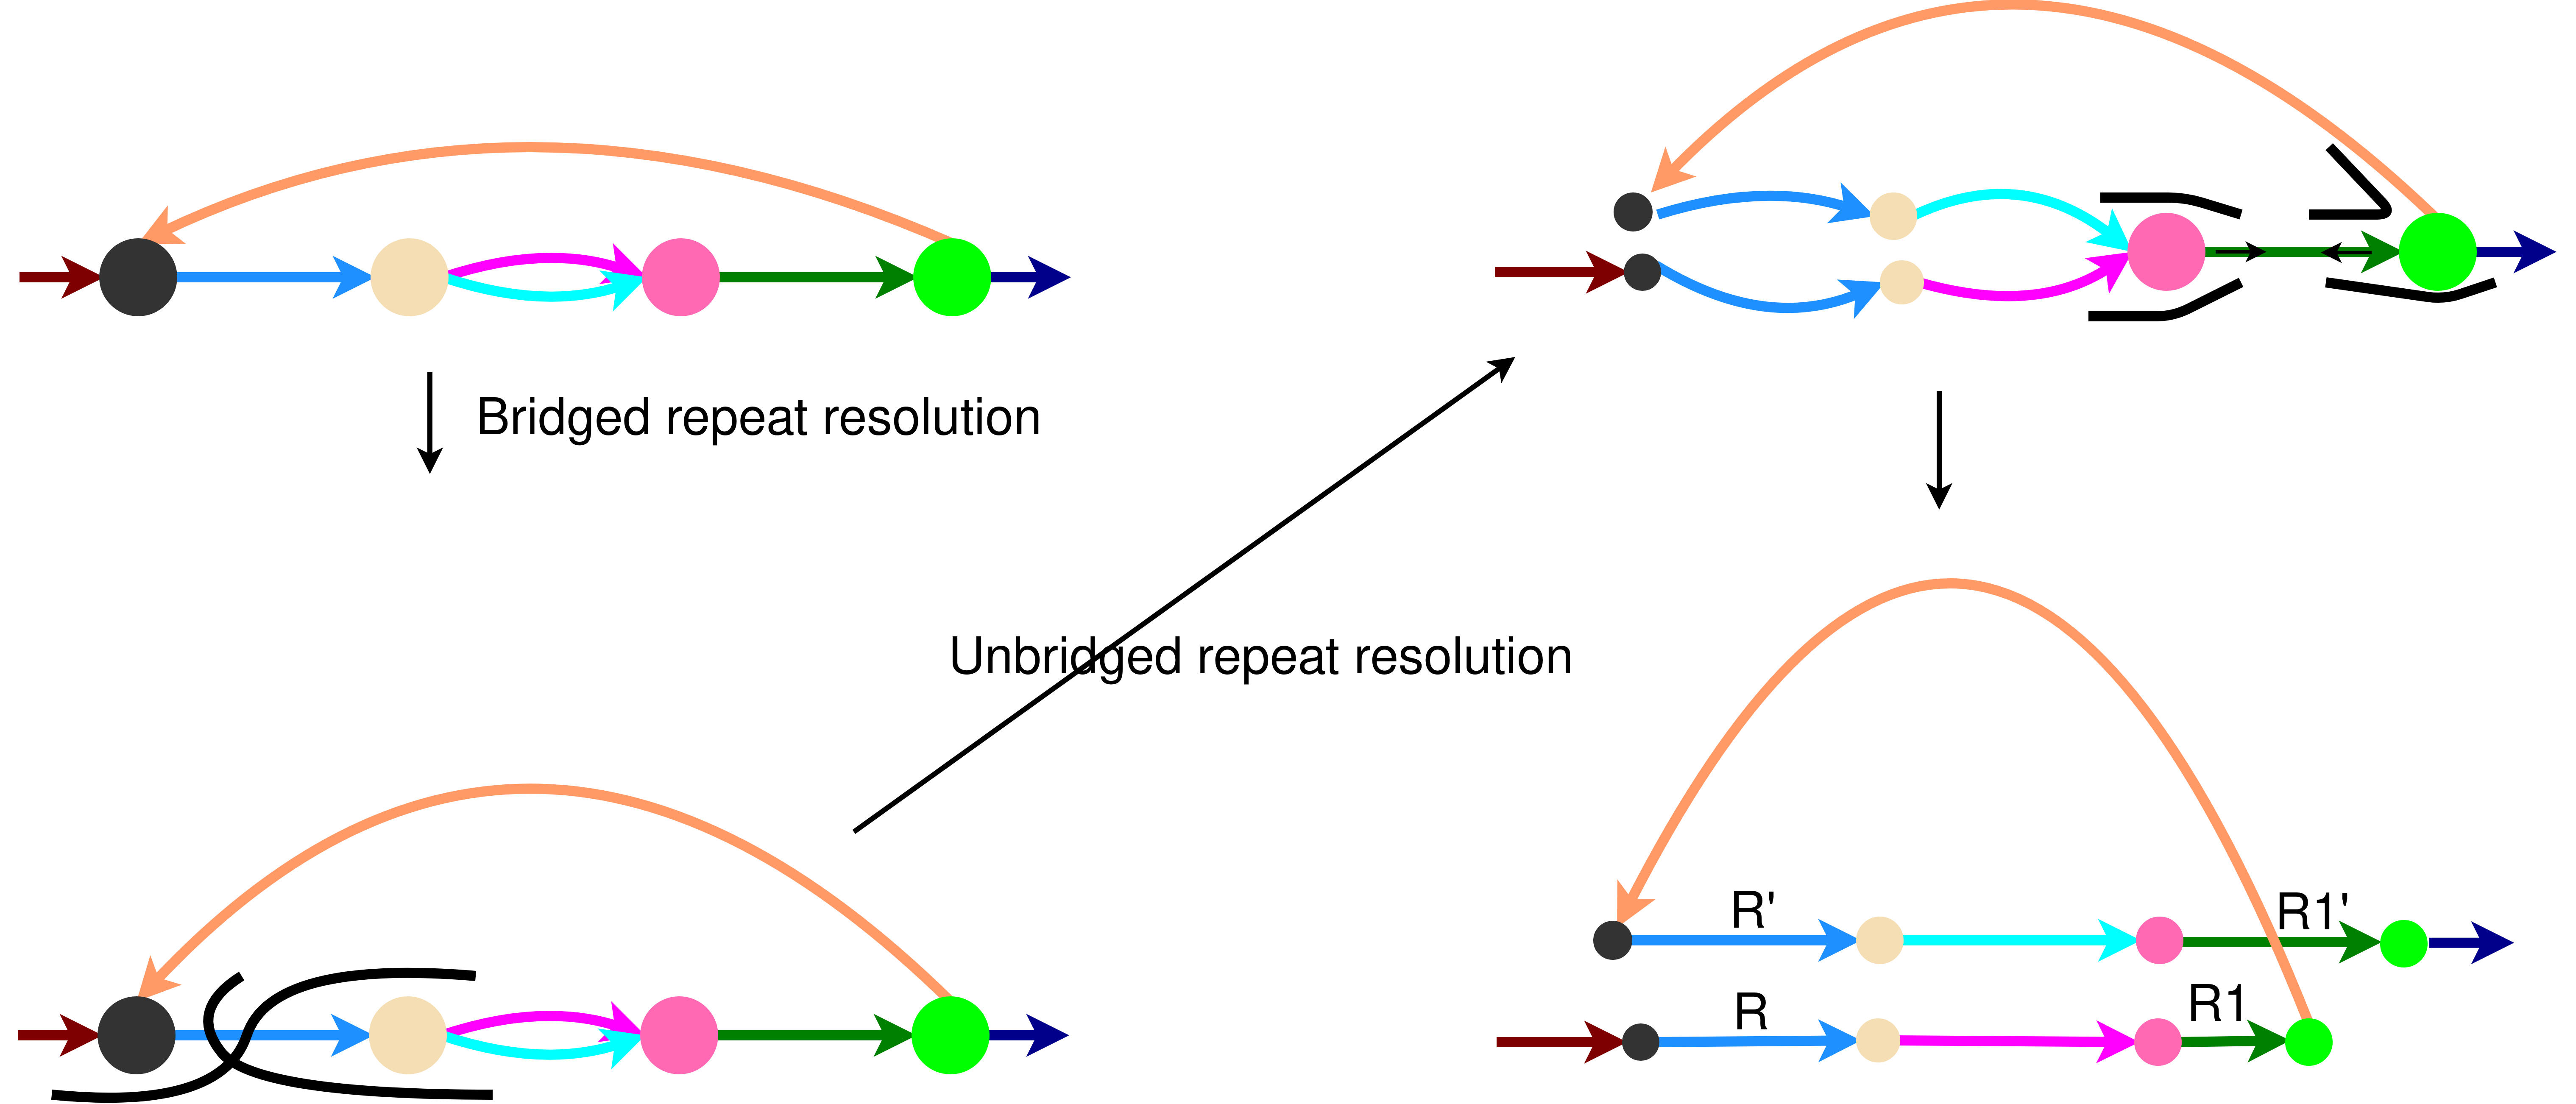
\includegraphics[width=11cm]{presentation/images/repeat_resolution.png}
      \caption*{Repeat resolution of the given example \cite{kolmogorov_assembly_2019}}
      \label{fig:contig_improvements}
    \end{figure}
    %From: 
    %https://www.youtube.com/watch?v=z6elrX-ZzW8&t=636s
    %(Youtube nanopore talk)
  \end{frame}

  \begin{frame}{Repeat resolution}
    "Pilon is a software tool which can be used to automatically improve draft assemblies or to find variation among strains, including large event detection. Pilon requires as input a FASTA file of the genome along with one or more BAM files of reads aligned to the input FASTA file. Pilon uses read alignment analysis to identify inconsistencies between the input genome and the evidence in the reads. It then attempts to make improvements to the input genome, including" \cite{walker_pilon_2014}:

    \begin{itemize}
      \item Single base differences
      \item Small indels
      \item Larger indel or block substitution events
      \item Gap filling
      \item Identification of local misassemblies, including optional opening of new gaps
    \end{itemize}
  \end{frame}

  \begin{frame}{Contigity improvement}
    \begin{figure}
      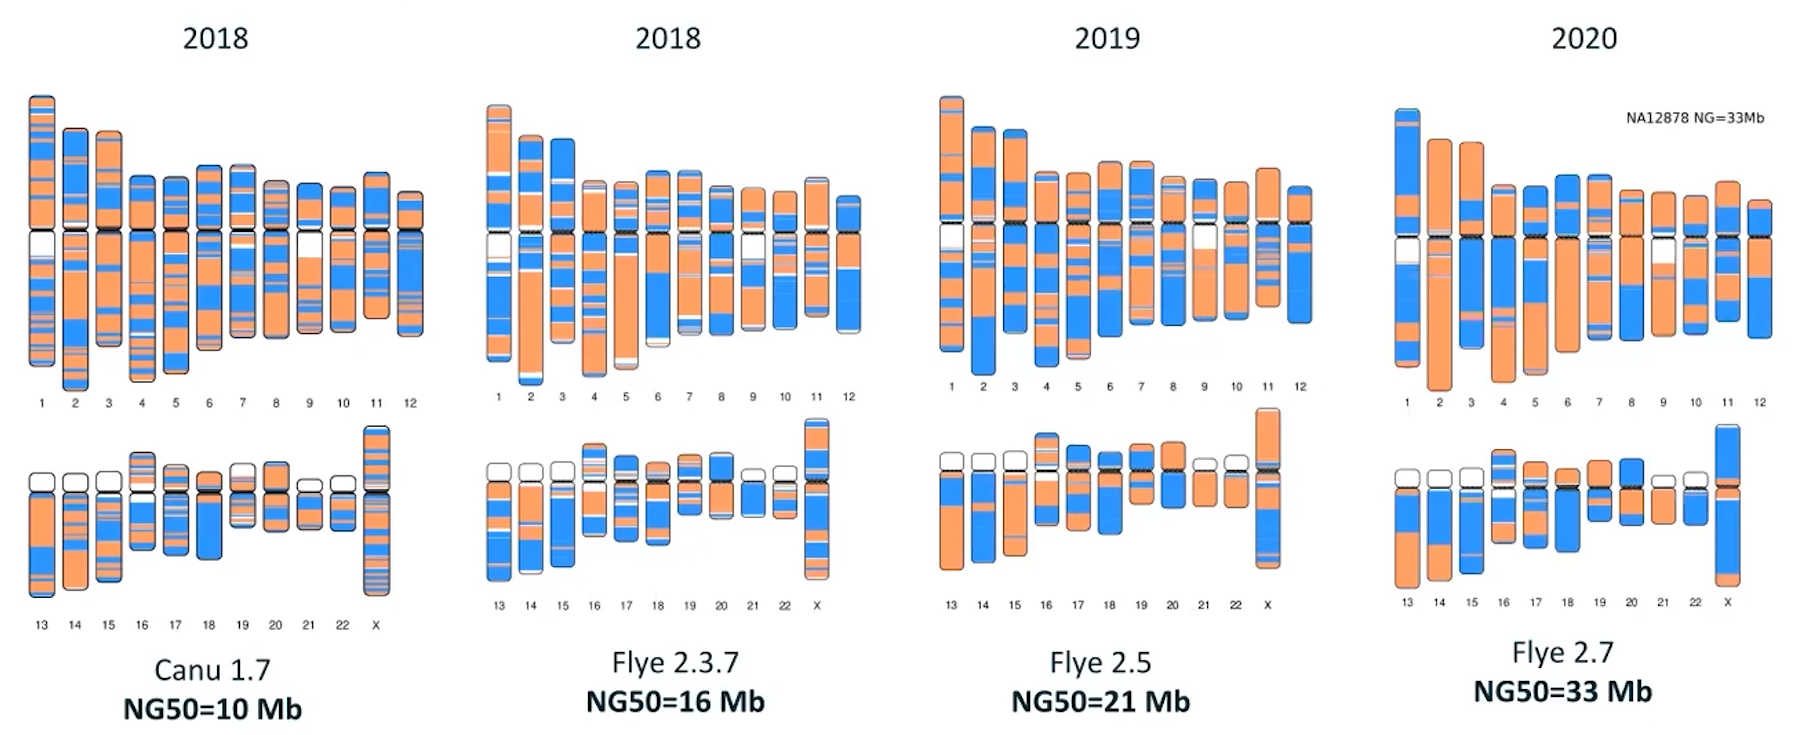
\includegraphics[width=11cm]{presentation/images/contigity_improvement.png}
      \caption*{Contigity improvements (M. Kolmogorov, personal communication, 29.07.2021)}
      \label{fig:contig_improvements}
    \end{figure}
    \begin{itemize}
      \item colors are contigs $\rightarrow$ change in color means fragmentation
    \end{itemize}
    %From: 
    %https://www.youtube.com/watch?v=z6elrX-ZzW8&t=636s
    %(Youtube nanopore talk)
  \end{frame}



\end{document}










